\documentclass[11pt]{article}

\usepackage[T1]{fontenc}
\usepackage{libertinus}
\usepackage{mathrsfs}
\usepackage{microtype}
\usepackage[a4paper,margin=27mm,headheight=14pt]{geometry}
\usepackage{amsmath,amssymb,amsthm,mathtools}
\usepackage{bm}
\usepackage{booktabs,longtable,tabularx,array,multirow}
\usepackage{enumitem}
\usepackage{graphicx}
\usepackage{xcolor}
\usepackage{listings}
\usepackage{fancyhdr}
\usepackage{hyperref}
\usepackage[nameinlink,noabbrev]{cleveref}
\usepackage{url}

\hypersetup{
  colorlinks=true,
  linkcolor=blue!45!black,
  citecolor=green!35!black,
  urlcolor=blue!55!black,
  pdftitle={Integral and Transform Frontiers for the Fabius--Rvachev System},
  pdfauthor={OpenAI GPT-5.6 Pro}
}

\pagestyle{fancy}
\fancyhf{}
\fancyhead[L]{Integral and Transform Frontiers}
\fancyhead[R]{Fabius--Rvachev System}
\fancyfoot[C]{\thepage}

\newtheorem{theorem}{Theorem}[section]
\newtheorem{proposition}[theorem]{Proposition}
\newtheorem{corollary}[theorem]{Corollary}
\newtheorem{lemma}[theorem]{Lemma}
\newtheorem{conjecture}[theorem]{Conjecture}
\theoremstyle{definition}
\newtheorem{definition}[theorem]{Definition}
\newtheorem{example}[theorem]{Example}
\newtheorem{problem}[theorem]{Research problem}
\theoremstyle{remark}
\newtheorem{remark}[theorem]{Remark}

\DeclareMathOperator{\upf}{up}
\DeclareMathOperator{\supp}{supp}
\DeclareMathOperator{\sinc}{sinc}
\DeclareMathOperator{\RePart}{Re}
\DeclareMathOperator{\Li}{Li}
\newcommand{\R}{\mathbb R}
\newcommand{\C}{\mathbb C}
\newcommand{\N}{\mathbb N}
\newcommand{\E}{\mathbb E}
\newcommand{\dd}{\,\mathrm d}
\newcommand{\ii}{\mathrm i}
\newcommand{\FF}{\mathscr F}
\newcommand{\Iop}{\mathcal I}
\newcommand{\Lap}{\mathcal L}
\newcommand{\Mell}{\mathcal M}
\newcommand{\fall}[2]{#1^{\underline{#2}}}
\newcommand{\Qm}{Q_m}
\newcommand{\An}{A_n}
\newcommand{\eps}{\varepsilon}
\newcommand{\abs}[1]{\lvert#1\rvert}
\newcommand{\norm}[1]{\lVert#1\rVert}
\newcommand{\set}[1]{\left\{#1\right\}}

\setlist[itemize]{topsep=3pt,itemsep=2pt,parsep=0pt}
\setlist[enumerate]{topsep=3pt,itemsep=2pt,parsep=0pt}
\setcounter{tocdepth}{2}

\title{\bfseries Integral and Transform Frontiers\\[2mm]
for the Fabius--Rvachev System}
\author{A repository-audited research report\\
\small prepared with symbolic derivations and reproducible numerical experiments}
\date{27 August 2026}

\begin{document}
\maketitle

\begin{abstract}
The Fabius function, its inverse, Rvachev's compactly supported \(\upf\)-function,
and the signed global self-differential extension form an unusually rigid calculus:
differentiation is conjugate to dyadic dilation.  This report develops the corresponding
\emph{integration} theory.  The first headline result is a two-sided integer
operator orbit
\[
  \mathrm D^r\FF(x)=2^{r(r+1)/2}\FF(2^r x),\qquad r\in\mathbb Z,
\]
where negative powers are the distinguished zero-initial antiderivatives.  It yields
closed forms for all integer-order primitives of \(F\), \(1-F\), and \(\upf\), and
finite formulas for polynomially weighted primitives.  Repeated integration by parts
then gives convergent series for arbitrary complex monomial powers, including negative
and fractional powers.

A second group of results concerns the inverse \(I=F^{-1}\).  In particular,
\[
  \int_0^y I(v)\,\dd v
  =yI(y)-F\!\left(\frac{I(y)}2\right),
\]
and integer powers \(I^m\) have finite closed primitives.  An entire Mellin
interpolant
\[
  D(z)=\int_0^1 x^zF'(x)\,\dd x
      =2^{-z}\sum_{j\ge0}\binom z{2j}c_j
\]
simultaneously represents all complex moments of the inverse:
\(D(z)=\int_0^1I(y)^z\dd y\).  This produces explicit rational-moment series for
negative powers and formulas for logarithmic inverse moments.

The strongest distributional result is an exact pushforward theorem.  If
\(Q_m=2^{m(m+1)/2}\), then for every \(m\ge1\),
\[
  \frac{\abs{F^{(m)}(U)}}{Q_m}\ \stackrel{d}{=}\ F(U),\qquad U\sim\mathrm{Unif}[0,1].
\]
Consequently all \(L^p\), Orlicz, Lorentz, and rearrangement-invariant norms of every
normalized derivative are known at once.  It also gives the sharp integrability law
\(I'\in L^p(0,1)\) exactly for \(0<p\le1\), together with an exact norm identity.

The report further develops Laplace, Fourier, Mellin, Cauchy--Stieltjes, correlation,
Riemann--Liouville, and Volterra-resolvent transforms.  The log-periodic factor already
present in the repository is used to prove a new obstruction: the integer
self-differential/dilation identity cannot extend exactly to a noninteger standard
fractional derivative.  Numerical experiments based on Fourier inversion verify the
new formulas to high precision.  Novelty claims are relative to the recursively audited
repository corpus, not assertions of worldwide priority.
\end{abstract}

\tableofcontents
\newpage

\section{Scope, corpus audit, and status of the results}

\subsection{Repository corpus and non-duplication boundary}

The recursive audit covered the LaTeX material under
\begin{center}
\url{https://github.com/VladimirReshetnikov/ProveIt/tree/main/Analysis/FabiusFunction/docs}.
\end{center}
The tree contains a current expository monograph, a merged research-frontier volume,
separate inverse-function and Newton--Rvachev reports, Thue--Morse and spectral reports,
Fourier-decay studies, archived predecessor drafts, a Lean walkthrough, a glossary,
and transcriptions of primary papers.  The live Newton--Rvachev report records a
67-source snapshot, while the archive explicitly preserves superseded and duplicated
versions.  Therefore the audit treated a current document and its archived ancestors as
one mathematical source rather than as independent evidence of novelty.

The corpus already develops, in depth:
\begin{itemize}
  \item the functional-differential equations, signed block extension, derivative
        formulae, partition of unity, and probabilistic random-series model;
  \item exact values at dyadic rationals, \(q\)-Pochhammer and \(q\)-binomial formulae,
        Thue--Morse cancellation, and moment recurrences;
  \item the infinite sinc/cosine Fourier products and sharp Fourier decay;
  \item endpoint asymptotics, Lambert--\(W\) saddle coordinates, periodic corrections,
        and Richardson-type acceleration;
  \item local inverse germs, inverse endpoint asymptotics, and formal series machinery;
  \item repeated integration as an approximation process converging to \(\upf\).
\end{itemize}

What was not found as a developed subject is a systematic calculus of indefinite
antiderivatives, polynomial/fractional weighted primitives, exact inverse-function
primitives, Mellin interpolation of inverse moments, derivative equimeasurability,
or the fractional-dilation obstruction proved here.  Some ingredients used below are
of course known in the repository---especially the derivative formula, block signs,
moments, Fourier product, and periodic Laplace factor.  The novelty lies in the new
integral consequences and their synthesis.

\begin{remark}[Priority discipline]
``New'' below means not duplicated in the inspected repository.  The report has not
performed an exhaustive search of every historical source in every language, so it does
not claim global first publication.  Each statement is marked as proved, conjectural,
or computationally supported.
\end{remark}

\subsection{Proof-status summary}

\begin{longtable}{p{0.34\textwidth}p{0.17\textwidth}p{0.40\textwidth}}
\toprule
Result family & Status & Main input \\
\midrule
\endhead
Two-sided integer derivative/primitive orbit & proved &
\(\FF'(x)=2\FF(2x)\), flatness at the origin \\
Polynomial and complex-power weighted primitives & proved &
finite/infinite integration by parts with flatness estimates \\
Closed primitive and power primitives of \(F^{-1}\) & proved &
change of variables \(y=F(x)\) and the primitive ladder \\
Fractional causal primitives and Volterra resolvent & proved &
Riemann--Liouville convolution and compact support \\
Laplace/Fourier/Mellin/Cauchy transform identities & proved &
probability model, integration by parts, moment expansion \\
Derivative pushforward/equimeasurability theorem & proved &
Thue--Morse block decomposition and exact sign balance \\
Sharp \(L^p\) threshold for \((F^{-1})'\) & proved &
pushforward theorem and endpoint flatness \\
No exact noninteger fractional-dilation collapse & proved &
periodic Laplace factor and nonzero first Fourier mode \\
Higher inverse-derivative \(L^p\) threshold & conjectural &
Lambert--\(W\) endpoint asymptotics and low-order formulas \\
Numerical constants and checks & computational &
FFT inversion of the infinite sinc product \\
\bottomrule
\end{longtable}

\subsection{Current Lean crosswalk for the normalized Volterra layer}

The proof labels above record the status of the report's mathematical arguments.  A later
implementation checkpoint now verifies the reusable operator layer: the declarations below
are present at compiled Lean commit \texttt{e109088ed}, verified by a focused build.  Put
\begin{equation}
 \mathsf J_{n,a}f(x):=
 \begin{cases}
 f(x),&n=0,\\[1mm]
 \displaystyle\frac1{(n-1)!}\int_a^x(x-t)^{n-1}f(t)\,\dd t,&n>0.
 \end{cases}                                                \label{eq:lean-volterra-current}
\end{equation}
The exact declarations in \path{FabiusFunction.NormalizedVolterra} are:
\begin{itemize}
\item \path{normalizedVolterra_affine}, the division-free identity
\begin{equation}
 \mathsf J_{n,ca+d}f(cx+d)
 =c^n\mathsf J_{n,a}\bigl(t\mapsto f(ct+d)\bigr)(x),          \label{eq:lean-affine-current}
\end{equation}
for every real \(c\), including \(c=0\) and negative scales, and including \(n=0\).  It
requires neither integrability nor completeness and works in any real normed target;
\item \path{normalizedVolterra_comp_affine}, the inverse-smul form
\begin{equation}
 \mathsf J_{n,a}\bigl(t\mapsto f(ct+d)\bigr)(x)
 =(c^n)^{-1}\mathsf J_{n,ca+d}f(cx+d),\qquad c\ne0,           \label{eq:lean-comp-affine-current}
\end{equation}
whose nonzero-scale hypothesis is required by the division;
\item \path{normalizedVolterra_basepoint_shift}, which, under interval integrability from
\(a\) to \(b\) and from \(b\) to \(x\), proves
\begin{equation}
 \mathsf J_{n,a}f(x)=\mathsf J_{n,b}f(x)
 +\sum_{k=0}^{n-1}\frac{(x-b)^k}{k!}\mathsf J_{n-k,a}f(b).    \label{eq:lean-basepoint-current}
\end{equation}
There is no ordering hypothesis on \(a,b,x\), and \(n=0\) is included;
\item \path{normalizedVolterra_succ_eq_taylor_of_eq_zero}, which assumes integrability only
from \(a\) to \(b\) and vanishing of \(f\) on the open unoriented interval between \(b\) and
\(x\), and proves
\begin{equation}
 \mathsf J_{n+1,a}f(x)
 =\sum_{k=0}^{n}\frac{(x-b)^k}{k!}\mathsf J_{n+1-k,a}f(b).    \label{eq:lean-zero-tail-current}
\end{equation}
It imposes neither endpoint values nor endpoint order; when \(b=x\), the vanishing condition
is vacuous.
\end{itemize}
Accordingly, the generic assertion that a positive-order Volterra primitive becomes a finite
Taylor polynomial after the input vanishes is Lean formalized.  Separately,
\path{normalizedVolterra_pow_mul_extendedFabius} and
\path{normalizedVolterra_pow_mul_fabiusReal_of_le_one} formalize the signed-global and
bounded-\(F\) natural-monomial coefficients, the latter on \(x\le1\).  The generic operator
theorem alone does not identify the displayed \(1-F\), shifted-\(\upf\), or exterior
piecewise moment coefficients; those report-specific evaluations retain their existing
paper-proof status.

\section{Normalization and structural identities}

\subsection{The three related functions}

Let \(F:[0,1]\to[0,1]\) be the standard Fabius distribution function, normalized by
\[
 F(0)=0,\qquad F(1)=1,\qquad F(1-x)=1-F(x).
\]
Its density can be written on the whole unit interval as
\begin{equation}
 F'(x)=2\upf(2x-1),\qquad 0\le x\le1.                 \label{eq:Fprime-up}
\end{equation}
The even, compactly supported Rvachev function is
\begin{equation}
 \upf(t)=
 \begin{cases}
   F(t+1),&-1\le t\le0,\\
   F(1-t),&0\le t\le1,\\
   0,&\abs{t}\ge1.
 \end{cases}                                             \label{eq:up-F}
\end{equation}
It is a probability density: \(\int_{-1}^1\upf(t)\dd t=1\).

The global signed self-differential extension is denoted by \(\FF\).  It agrees with
\(F\) on \([0,1]\), vanishes on \(( -\infty,0]\), and satisfies
\begin{equation}
 \FF'(x)=2\FF(2x).                                      \label{eq:global-selfdiff}
\end{equation}
Writing \(\eps_k=(-1)^{s_2(k)}\), where \(s_2(k)\) is the binary digit sum, its block
form is
\begin{equation}
 \FF(x)=\eps_k\upf(x-2k-1),\qquad 2k\le x\le2k+2.       \label{eq:block}
\end{equation}
The first \(2^r\) Thue--Morse signs have equally many plus and minus signs whenever
\(r\ge1\).

\subsection{Derivatives, moments, and transforms already available}

Iteration of \eqref{eq:global-selfdiff} gives
\begin{equation}
 \FF^{(m)}(x)=Q_m\FF(2^m x),\qquad
 Q_m:=2^{m(m+1)/2}.                                      \label{eq:derivative-orbit}
\end{equation}
All derivatives of \(F\) vanish at both endpoints.  Define the even moments
\begin{equation}
 c_j:=\int_{-1}^1t^{2j}\upf(t)\dd t.                     \label{eq:cj}
\end{equation}
They are rational and begin
\[
 c_0=1,\qquad c_1=\frac19,\qquad c_2=\frac{19}{675},\ldots.
\]
With the Fourier convention
\(
 \widehat f(\xi)=\int_\R f(x)e^{-2\pi\ii x\xi}\dd x,
\)
\begin{equation}
 \widehat{\upf}(\xi)
 =\prod_{n=0}^{\infty}\sinc\!\left(\frac{\pi\xi}{2^n}\right)
 =\prod_{m=1}^{\infty}\cos\!\left(\frac{\pi\xi}{2^m}\right)^m. \label{eq:up-fourier}
\end{equation}
The bilateral moment-generating transform is
\begin{equation}
 M(s):=\int_{-1}^1e^{st}\upf(t)\dd t
 =\prod_{j=1}^{\infty}\frac{\sinh(s/2^j)}{s/2^j}.        \label{eq:M-product}
\end{equation}
These established identities are the raw material for the integration theory below.

\section{The exact antiderivative ladder}

\subsection{A two-sided integer differential orbit}

For \(n\ge1\), put
\begin{equation}
 A_n:=2^{n(n-1)/2}.                                      \label{eq:An}
\end{equation}
Notice that \(A_n=Q_n/2^n\).

\begin{theorem}[Distinguished \(n\)-fold primitive of the global extension]
\label{thm:global-primitive}
For \(x\ge0\) and \(n\ge1\),
\begin{equation}
 \frac1{(n-1)!}\int_0^x(x-t)^{n-1}\FF(t)\dd t
 =A_n\FF\!\left(\frac{x}{2^n}\right).                  \label{eq:global-primitive}
\end{equation}
Equivalently, with zero-initial negative powers of differentiation,
\begin{equation}
 \boxed{\quad
 \mathrm D^r\FF(x)=2^{r(r+1)/2}\FF(2^r x),
 \qquad r\in\mathbb Z.
 \quad}                                                  \label{eq:integer-orbit}
\end{equation}
\end{theorem}

\begin{proof}
For positive \(r\), this is \eqref{eq:derivative-orbit}.  For \(r=-n\), differentiate
\(A_n\FF(x/2^n)\) exactly \(n\) times.  The chain rule and
\eqref{eq:derivative-orbit} give the coefficient
\[
 A_n2^{-n^2}Q_n
 =2^{n(n-1)/2-n^2+n(n+1)/2}=1,
\]
so the \(n\)-th derivative is \(\FF(x)\).  Every derivative of the proposed primitive
of order below \(n\) vanishes at \(x=0\), because \(\FF\) is flat there.  These are
precisely the initial conditions characterizing the Volterra integral on the left.
\end{proof}

\begin{corollary}[All local primitives of \(F\)]
\label{cor:F-primitives}
On \([0,1]\), every \(n\)-fold indefinite primitive of \(F\) is
\begin{equation}
 \mathrm D^{-n}F(x)=A_nF\!\left(\frac{x}{2^n}\right)+P_{n-1}(x), \label{eq:F-nprimitive}
\end{equation}
where \(P_{n-1}\) is an arbitrary polynomial of degree at most \(n-1\).  The
zero-initial primitive is the first term alone.
\end{corollary}

The first cases are exceptionally simple:
\begin{align}
 \int_0^xF(t)\dd t&=F(x/2),                                      \label{eq:F-first-primitive}\\
 \int_0^x(x-t)F(t)\dd t&=2F(x/4),                                \\
 \frac12\int_0^x(x-t)^2F(t)\dd t&=8F(x/8).
\end{align}
Thus the antiderivatives are not merely expressible by quadrature: they remain in the
same self-differential orbit.

\begin{corollary}[Primitives of \(\upf\), \(1-F\), and affine copies]
\label{cor:other-primitives}
For \(-1\le x\le1\),
\begin{equation}
 \frac1{(n-1)!}\int_{-1}^x(x-t)^{n-1}\upf(t)\dd t
 =A_nF\!\left(\frac{x+1}{2^n}\right).                    \label{eq:up-local-primitive}
\end{equation}
For \(0\le x\le1\),
\begin{equation}
 \mathrm D^{-n}(1-F(x))
 =(-1)^nA_nF\!\left(\frac{1-x}{2^n}\right)+P_{n-1}(x).   \label{eq:one-minus-F}
\end{equation}
More generally, for \(a\ne0\), on every interval where the relevant global branch is fixed,
\begin{equation}
 \mathrm D^{-n}F(ax+b)
 =a^{-n}A_n\FF\!\left(\frac{ax+b}{2^n}\right)+P_{n-1}(x). \label{eq:affine-primitive}
\end{equation}
The condition \(a\ne0\) is required by this inverse-scaled formula.  It is distinct from the
division-free forward covariance \eqref{eq:lean-affine-current}, which remains valid when the
scale is zero.
\end{corollary}

\begin{proof}
For \eqref{eq:up-local-primitive}, differentiating the right side \(n\) times gives
\(\FF(x+1)=\upf(x)\) on \([-1,1]\).  Formula \eqref{eq:one-minus-F} follows from
\(1-F(x)=F(1-x)\).  The affine formula is the chain rule for \(a\ne0\).
\end{proof}

\subsection{Global causal primitives of \(\upf\)}

The scaled formula \eqref{eq:up-local-primitive} is local because \(\FF(x+1)\) ceases
to equal \(\upf(x)\) outside its central block.  The global causal primitive becomes a
moment polynomial after the support is passed.

\begin{proposition}[Complete piecewise form]
\label{prop:up-causal}
Let
\[
 U_n(x):=\frac1{(n-1)!}\int_{-1}^{x}(x-t)^{n-1}\upf(t)\dd t,
\]
with the upper limit understood as \(\min(x,1)\) once \(x>1\).  Then
\begin{equation}
 U_n(x)=
 \begin{cases}
  0,&x\le-1,\\[1mm]
  A_nF((x+1)/2^n),&-1\le x\le1,\\[1mm]
  \displaystyle
  \frac1{(n-1)!}
  \sum_{j=0}^{\lfloor(n-1)/2\rfloor}
    \binom{n-1}{2j}c_jx^{n-1-2j},&x\ge1.
 \end{cases}                                               \label{eq:up-causal-piecewise}
\end{equation}
\end{proposition}

\begin{proof}
Only the last branch needs comment.  Expand \((x-t)^{n-1}\); odd moments vanish by
evenness of \(\upf\), and the even moments are \(c_j\).
\end{proof}

\begin{remark}[Formal status of the zero tail]
At compiled checkpoint \texttt{e109088ed}, the declaration
\begin{center}
\path{normalizedVolterra_succ_eq_taylor_of_eq_zero}
\end{center}
formally supplies the generic finite Taylor polynomial once the integrand vanishes beyond
the support.  It does not by itself prove the explicit \(c_j\)-coefficient identification in
\eqref{eq:up-causal-piecewise}, nor the analogous displayed \(F\)- or
\(\upf\)-specific coefficients; those specializations remain at the report's paper-proof
status.
\end{remark}

\subsection{Definite dyadic integrals become exact arithmetic}

A direct endpoint consequence is useful for the arithmetic side of the repository.

\begin{corollary}[Polynomial integrals over dyadic intervals]
If \(P\in\mathbb Q[x]\) and \(a,b\in[0,1]\) are dyadic rationals, then
\(
 \int_a^bP(x)F(x)\dd x
\)
is rational.  The same holds for \(P(x)\upf(x)\) on dyadic subintervals of
\([-1,1]\).
\end{corollary}

\begin{proof}
The finite endpoint formula in \cref{thm:polynomial-primitive} below involves only
rational coefficients and values of \(F\) at dyadic arguments.  Those values are
rational by the established arithmetic theory.
\end{proof}

This creates a direct bridge from antiderivatives to the repository's
\(q\)-binomial formulae: every such integral can be converted into a finite expression
in exactly computable dyadic values and then into the preferred \(q\)-arithmetic form.

\section{Polynomial, analytic, fractional, and negative weights}

\subsection{A finite operator formula for every polynomial weight}

Define the zero-initial primitive ladder
\begin{equation}
 \mathcal A_j(x):=A_jF(x/2^j),\qquad j\ge1,                \label{eq:Aj-ladder}
\end{equation}
so \(\mathcal A_j'=\mathcal A_{j-1}\), with
\(\mathcal A_0=F\).

\begin{theorem}[Polynomially weighted \(n\)-fold primitives]
\label{thm:polynomial-primitive}
Let \(P\) be a polynomial of degree \(d\), and let \(n\ge1\).  Then
\begin{equation}
 \boxed{
 \frac1{(n-1)!}\int_0^x(x-t)^{n-1}P(t)F(t)\dd t
 =\sum_{k=0}^{d}(-1)^k\binom{n+k-1}{k}
   P^{(k)}(x)\mathcal A_{n+k}(x).
 }                                                        \label{eq:poly-nfold}
\end{equation}
Consequently the general indefinite \(n\)-fold primitive is the right side plus an
arbitrary polynomial of degree at most \(n-1\).
\end{theorem}

\begin{proof}
Differentiate the right side.  The contributions containing \(P^{(k)}\mathcal
A_{n+k-1}\) cancel by Pascal's identity.  Repeating this \(n\) times leaves
\(P(x)F(x)\).  Every derivative of order below \(n\) vanishes at the origin because all
members of the \(\mathcal A\)-ladder are flat there.  This identifies the Volterra
solution uniquely.
\end{proof}

For a monomial \(P(x)=x^p\), \(p\in\N\), the formula is
\begin{equation}
 \frac1{(n-1)!}\int_0^x(x-t)^{n-1}t^pF(t)\dd t
 =\sum_{k=0}^{p}(-1)^k\binom{n+k-1}{k}
   \frac{p!}{(p-k)!}x^{p-k}A_{n+k}F(x/2^{n+k}).            \label{eq:monomial-nfold}
\end{equation}
In particular,
\begin{equation}
 \int_0^1x^pF(x)\dd x
 =\sum_{k=0}^{p}(-1)^k\frac{p!}{(p-k)!}
   2^{k(k+1)/2}F(2^{-k-1}).                               \label{eq:integer-moment-F}
\end{equation}
This is a finite rational closed form.  The first examples are
\begin{equation}
 \int_0^1F(x)\dd x=\frac12,\qquad
 \int_0^1xF(x)\dd x=\frac{13}{36},\qquad
 \int_0^1x^2F(x)\dd x=\frac5{18}.                        \label{eq:first-F-moments}
\end{equation}
Since \(\upf(x)=1-F(x)\) on \([0,1]\),
\begin{equation}
 \int_0^1x^p\upf(x)\dd x
 =\frac1{p+1}-\int_0^1x^pF(x)\dd x.                      \label{eq:half-up-moments}
\end{equation}
Formula \eqref{eq:half-up-moments} is compatible with the half-moment sequences already
studied in the repository; the new contribution here is the finite antiderivative route.

\subsection{Convergent series for arbitrary complex powers}

For \(\alpha\in\C\), write
\(
 \fall{\alpha}{k}=\alpha(\alpha-1)\cdots(\alpha-k+1)
\)
and use the real logarithm to define \(x^\alpha=e^{\alpha\log x}\) for \(x>0\).

\begin{theorem}[Complex-power weighted primitive]
\label{thm:complex-power}
For every \(\alpha\in\C\), every integer \(n\ge1\), and every \(x>0\),
\begin{equation}
 \boxed{
 \frac1{(n-1)!}\int_0^x(x-t)^{n-1}t^\alpha F(t)\dd t
 =\sum_{k=0}^{\infty}(-1)^k\binom{n+k-1}{k}
   \fall{\alpha}{k}x^{\alpha-k}\mathcal A_{n+k}(x).
 }                                                        \label{eq:complex-power-series}
\end{equation}
The integral and series are locally uniform entire functions of \(\alpha\).  If
\(\alpha\in\N\), the series terminates and reduces to
\eqref{eq:monomial-nfold}.  Negative and fractional powers require no endpoint
regularization because \(F\) is flat at zero.
\end{theorem}

\begin{proof}
Repeated integration by parts gives the first \(N\) terms and a remainder containing
\(\fall{\alpha}{N+1}\) times a higher primitive.  Flatness implies that for every
integer \(r\ge0\) there is \(C_r\) such that \(0\le F(t)\le C_rt^r\) on \([0,x]\).
Consequently
\begin{equation}
 0\le\mathcal A_m(x)
 \le C_r\frac{r!\,x^{m+r}}{(m+r)!}.                       \label{eq:primitive-flat-bound}
\end{equation}
The factorial in the denominator dominates the falling factorial and the polynomial
factor \(\binom{n+k-1}{k}\); choosing \(r\) large gives absolute, locally uniform
convergence and sends the remainder to zero.  The same bound permits differentiation
with respect to \(\alpha\).
\end{proof}

The first-order case is especially transparent:
\begin{equation}
 \int_0^xt^\alpha F(t)\dd t
 =\sum_{k=0}^{\infty}(-1)^k\fall{\alpha}{k}
   x^{\alpha-k}2^{k(k+1)/2}F(x/2^{k+1}).                  \label{eq:complex-first-primitive}
\end{equation}
It is a convergent self-similar transseries whose scales descend geometrically while its
coefficients grow factorially; endpoint flatness makes the net terms summable.

\subsection{Analytic weights and exponential resolvents}

The same argument applies to a sufficiently controlled analytic weight \(g\):
\begin{equation}
 \Iop^n(gF)(x)
 =\sum_{k=0}^{\infty}(-1)^k\binom{n+k-1}{k}
   g^{(k)}(x)\mathcal A_{n+k}(x),                          \label{eq:analytic-weight}
\end{equation}
provided the derivative growth is dominated by the factorial decay in
\eqref{eq:primitive-flat-bound}.  For \(g(x)=e^{\lambda x}\), this gives the entire
series
\begin{equation}
 \Iop^n(e^{\lambda x}F(x))
 =e^{\lambda x}\sum_{k=0}^{\infty}(-\lambda)^k
   \binom{n+k-1}{k}A_{n+k}F(x/2^{n+k}).                   \label{eq:exponential-weight}
\end{equation}
This is a local resolvent expansion entirely in scaled Fabius values.

\section{Closed primitives involving the inverse Fabius function}

Let
\begin{equation}
 I:=F^{-1}:(0,1)\to(0,1).                                 \label{eq:inverse-def}
\end{equation}
It obeys \(I(1-y)=1-I(y)\) and
\begin{equation}
 I'(y)=\frac1{F'(I(y))}.                                  \label{eq:inverse-derivative}
\end{equation}

\subsection{A closed first primitive}

\begin{theorem}[Exact area primitive of the inverse]
\label{thm:inverse-primitive}
For \(0\le y\le1\),
\begin{equation}
 \boxed{
 \int_0^y I(v)\dd v
 =yI(y)-F\!\left(\frac{I(y)}2\right).
 }                                                        \label{eq:inverse-primitive-closed}
\end{equation}
Thus an indefinite primitive is
\(
 yI(y)-F(I(y)/2)+C.
\)
\end{theorem}

\begin{proof}
Put \(q=I(y)\), change variables \(v=F(x)\), and integrate by parts:
\[
 \int_0^yI(v)\dd v
 =\int_0^q xF'(x)\dd x
 =qy-\int_0^qF(x)\dd x.
\]
The final integral is \(F(q/2)\) by \eqref{eq:F-first-primitive}.
\end{proof}

At \(y=1/2\), \(I(y)=1/2\), and \(F(1/4)=5/72\), so
\begin{equation}
 \int_0^{1/2}I(v)\dd v=\frac14-\frac5{72}=\frac{13}{72}. \label{eq:inverse-half-area}
\end{equation}
At \(y=1\), the formula gives \(\int_0^1I=1/2\), as required by symmetry.

\subsection{Powers of the inverse}

\begin{theorem}[Primitive of an arbitrary complex inverse power]
\label{thm:inverse-power-primitive}
For \(\alpha\in\C\), \(0<y<1\), and \(q=I(y)\),
\begin{align}
 \int_0^yI(v)^\alpha\dd v
 &=yq^\alpha-\alpha\int_0^qx^{\alpha-1}F(x)\dd x          \label{eq:inverse-power-basic}\\
 &=yq^\alpha-\alpha\sum_{k=0}^{\infty}(-1)^k
   \fall{\alpha-1}{k}q^{\alpha-1-k}
   2^{k(k+1)/2}F(q/2^{k+1}).                              \label{eq:inverse-power-series}
\end{align}
The series terminates when \(\alpha\) is a nonnegative integer.
\end{theorem}

\begin{proof}
After \(v=F(x)\), integrate \(x^\alpha F'(x)\) by parts.  The boundary term at zero
vanishes for every complex \(\alpha\) because \(F\) is flatter than every power.  Then
apply \cref{thm:complex-power} with exponent \(\alpha-1\).
\end{proof}

For \(m\in\N\), this is the finite closed form
\begin{equation}
 \int_0^yI(v)^m\dd v
 =yq^m-m\sum_{k=0}^{m-1}(-1)^k
   \frac{(m-1)!}{(m-1-k)!}q^{m-1-k}
   2^{k(k+1)/2}F(q/2^{k+1}).                              \label{eq:inverse-integer-power}
\end{equation}

\subsection{All repeated primitives: a layer-cake formula}

\begin{theorem}[\(n\)-fold primitive of an inverse power]
\label{thm:inverse-nfold}
For \(n\ge1\), \(\RePart\alpha>0\), and \(q=I(y)\),
\begin{equation}
 \frac1{(n-1)!}\int_0^y(y-v)^{n-1}I(v)^\alpha\dd v
 =\frac{\alpha}{n!}\int_0^q x^{\alpha-1}(y-F(x))^n\dd x. \label{eq:inverse-nfold}
\end{equation}
In particular,
\begin{equation}
 \frac1{(n-1)!}\int_0^y(y-v)^{n-1}I(v)\dd v
 =\frac1{n!}\int_0^{I(y)}(y-F(x))^n\dd x.                \label{eq:inverse-nfold-alpha1}
\end{equation}
\end{theorem}

\begin{proof}
Use
\(
 I(v)^\alpha=\int_0^{I(v)}\alpha x^{\alpha-1}\dd x
\).  For real \(\alpha>0\), Tonelli's theorem applies directly; for complex
\(\RePart\alpha>0\), absolute convergence gives Fubini's theorem (or equivalently
analytic continuation from the positive real axis).  The condition \(x<I(v)\) is equivalent to \(F(x)<v\).  The
inner integral is
\(
 (n-1)!^{-1}\int_{F(x)}^y(y-v)^{n-1}\dd v=(y-F(x))^n/n!.
\)
\end{proof}

Expansion of the right side gives a finite reduction to integrals of
\(x^{\alpha-1}F(x)^k\).  It also provides a stable numerical representation near the
singular endpoints, where direct differentiation of \(I\) is ill-conditioned.

\subsection{A general weighted area identity}

For every integrable weight \(w\), Fubini gives
\begin{equation}
 \int_0^1w(y)I(y)\dd y
 =\int_0^1\left(\int_{F(x)}^1w(y)\dd y\right)\dd x.        \label{eq:weighted-area-inverse}
\end{equation}
With \(w(y)=y^n\),
\begin{equation}
 \int_0^1y^nI(y)\dd y
 =\frac{1-\int_0^1F(x)^{n+1}\dd x}{n+1}.                 \label{eq:inverse-y-moment}
\end{equation}
This converts mixed quantile moments into nonlinear Fabius moments without numerical
inversion.

\section{Causal fractional integrals and the Volterra resolvent}

\subsection{Riemann--Liouville primitives of \(\upf\)}

For \(\beta>0\), define
\begin{equation}
 U_\beta(x):=\frac1{\Gamma(\beta)}
 \int_{-1}^{\min(x,1)}(x-t)^{\beta-1}\upf(t)\dd t,
 \qquad x>-1.                                             \label{eq:fractional-up}
\end{equation}
For integer \(\beta=n\), this is \cref{prop:up-causal}.

\begin{proposition}[Transform and tail expansion]
\label{prop:fractional-up-transform}
Let \(V_\beta(y)=U_\beta(y-1)\), \(y>0\).  For \(\RePart s>0\),
\begin{equation}
 \Lap[V_\beta](s)=s^{-\beta}e^{-s}M(s).                   \label{eq:fractional-up-laplace}
\end{equation}
For \(x>1\),
\begin{equation}
 U_\beta(x)=\frac{x^{\beta-1}}{\Gamma(\beta)}
 \sum_{j=0}^{\infty}\binom{\beta-1}{2j}\frac{c_j}{x^{2j}}. \label{eq:fractional-tail}
\end{equation}
The series also converges at \(x=1\), because \(\upf\) is flat at both support
endpoints.  When \(\beta\) is a positive integer it terminates, recovering the moment
polynomial in \eqref{eq:up-causal-piecewise}.
\end{proposition}

\begin{proof}
After shifting the support to \([0,2]\), the transform of the density is
\(e^{-s}M(-s)=e^{-s}M(s)\).  Riemann--Liouville integration multiplies the Laplace
transform by \(s^{-\beta}\).  For the tail, expand
\((x-t)^{\beta-1}\) in powers of \(t/x\); odd moments vanish.  Endpoint flatness gives
termwise convergence at the boundary case \(x=1\).
\end{proof}

The semigroup law
\begin{equation}
 U_{\alpha+\beta}=\Iop^\alpha U_\beta                 \label{eq:fractional-semigroup}
\end{equation}
follows from the beta integral.  This gives a natural continuous interpolation between
the exact integer primitives, although \cref{sec:fractional-obstruction} shows that it
cannot collapse to one simply scaled Fabius function at noninteger order.

\subsection{Volterra resolvent}

For \(\lambda\in\C\), define
\begin{equation}
 R_\lambda(x):=\int_{-1}^{\min(x,1)}e^{\lambda(x-t)}\upf(t)\dd t. \label{eq:resolvent-def}
\end{equation}

\begin{theorem}[Resolvent series]
\label{thm:resolvent}
The function \(R_\lambda\) is entire in \(\lambda\) and
\begin{equation}
 R_\lambda(x)=\sum_{n=1}^{\infty}\lambda^{n-1}U_n(x).     \label{eq:resolvent-series}
\end{equation}
On the support interval,
\begin{equation}
 R_\lambda(x)=\sum_{n=1}^{\infty}\lambda^{n-1}
 A_nF((x+1)/2^n),\qquad -1\le x\le1.                     \label{eq:resolvent-F-series}
\end{equation}
It is the unique solution of
\begin{equation}
 R_\lambda'(x)=\upf(x)+\lambda R_\lambda(x),\qquad R_\lambda(-1)=0. \label{eq:resolvent-ode}
\end{equation}
For \(x\ge1\),
\begin{equation}
 R_\lambda(x)=e^{\lambda x}M(\lambda).                   \label{eq:resolvent-tail}
\end{equation}
\end{theorem}

At \(x=1\), this yields the scale-value/product identity
\begin{equation}
 e^\lambda M(\lambda)
 =\sum_{n=1}^{\infty}\lambda^{n-1}
   2^{n(n-1)/2}F(2^{1-n}).                                \label{eq:resolvent-product-identity}
\end{equation}
It is an entire generating function for inverse-dyadic Fabius values at a different
normalization from the usual moment generating series.

\section{Laplace and Fourier transforms on the unit interval}

\subsection{Closed transforms of \(F\) and the positive half of \(\upf\)}

\begin{theorem}[One-sided exponential transforms]
\label{thm:one-sided-laplace}
For \(s\in\C\setminus\{0\}\),
\begin{align}
 \int_0^1e^{sx}F(x)\dd x
 &=\frac{e^s-e^{s/2}M(s/2)}{s},                           \label{eq:F-laplace}\\
 \int_0^1e^{sx}\upf(x)\dd x
 &=\frac{e^{s/2}M(s/2)-1}{s}.                             \label{eq:up-half-laplace}
\end{align}
The removable values at \(s=0\) are both \(1/2\).
\end{theorem}

\begin{proof}
Integration by parts gives
\[
 s\int_0^1e^{sx}F(x)\dd x=e^s-\int_0^1e^{sx}F'(x)\dd x.
\]
With \(t=2x-1\), \eqref{eq:Fprime-up} turns the last integral into
\(e^{s/2}M(s/2)\).  The second formula follows from \(\upf(x)=1-F(x)\) on
\([0,1]\).
\end{proof}

Setting \(s=-2\pi\ii\xi\) gives a one-sided Fourier transform not explicit in the
repository's full-line \(\upf\) product:
\begin{equation}
 \int_0^1F(x)e^{-2\pi\ii\xi x}\dd x
 =\frac{e^{-2\pi\ii\xi}-e^{-\pi\ii\xi}\widehat{\upf}(\xi/2)}
 {-2\pi\ii\xi}.                                          \label{eq:F-fourier-one-sided}
\end{equation}
The transform of the positive half of \(\upf\) is obtained by replacing the numerator
with \(e^{-\pi\ii\xi}\widehat{\upf}(\xi/2)-1\).

\subsection{A Bromwich-compatible primitive representation}

Use the conventional one-sided Laplace transform
\(
 \Lap_-[f](s)=\int_0^\infty e^{-st}f(t)\dd t
\).
Equation \eqref{eq:F-laplace}, with \(s\mapsto-s\), gives
\begin{equation}
 \Lap_-[F\mathbf{1}_{[0,1]}](s)
 =\frac{e^{-s/2}M(s/2)-e^{-s}}{s}.                         \label{eq:F-conventional-Laplace}
\end{equation}
For \(0<x<1\) and any admissible Bromwich line \(\RePart s=c>0\), the causal primitive
therefore has the representation
\begin{equation}
 \mathcal A_n(x)
 =\frac1{2\pi\ii}\int_{c-\ii\infty}^{c+\ii\infty}
   e^{sx}s^{-n}\Lap_-[F\mathbf{1}_{[0,1]}](s)\dd s.         \label{eq:Bromwich-primitive}
\end{equation}
The exact scaled formula \(\mathcal A_n(x)=A_nF(x/2^n)\) is thus a nontrivial collapse
of a Bromwich integral on the unit interval.  At fractional order, the analogous
global collapse fails by the periodic obstruction in \cref{sec:fractional-obstruction}.

\section{An entire Mellin interpolant and inverse moments}

\subsection{Definition and binomial moment expansion}

Define
\begin{equation}
 D(z):=\int_0^1x^zF'(x)\dd x.                             \label{eq:D-def}
\end{equation}
Because \(F'\) is flat at zero, the integral converges locally uniformly for every
\(z\in\C\); hence \(D\) is entire.

\begin{theorem}[Entire binomial-moment interpolation]
\label{thm:D-series}
For all \(z\in\C\),
\begin{equation}
 \boxed{
 D(z)=\int_{-1}^1\left(\frac{1+t}{2}\right)^z\upf(t)\dd t
 =2^{-z}\sum_{j=0}^{\infty}\binom z{2j}c_j.
 }                                                        \label{eq:D-series}
\end{equation}
The series converges locally uniformly on \(\C\).  At nonnegative integers, \(D(n)\)
is the usual Fabius-distribution moment and the series terminates.
\end{theorem}

\begin{proof}
The first equality follows from \(t=2x-1\) in \eqref{eq:Fprime-up}.  Expand
\((1+t)^z\) binomially.  Odd terms integrate to zero.  Although the binomial series has
boundary radius one, the moments \(c_j\) decay faster than every power because \(\upf\)
is flat at \(\abs{t}=1\); this gives local uniform convergence after integration.
\end{proof}

For a positive integer \(m\),
\begin{equation}
 D(-m)=2^m\sum_{j=0}^{\infty}
 \binom{m+2j-1}{2j}c_j.                                  \label{eq:D-negative-integer}
\end{equation}
Thus every negative inverse moment is represented by a rapidly convergent positive
series of rational terms.

\subsection{Mellin transforms of \(F\) and \(\upf\)}

Let
\begin{equation}
 H(z):=\int_0^1x^{z-1}F(x)\dd x.                          \label{eq:H-def}
\end{equation}
Flatness again makes \(H\) entire.  Integration by parts gives
\begin{equation}
 \boxed{H(z)=\frac{1-D(z)}{z}},                            \label{eq:H-D}
\end{equation}
where \(z=0\) is removable.  For \(m\ge1\),
\begin{equation}
 \int_0^1x^{-m-1}F(x)\dd x=\frac{D(-m)-1}{m}.            \label{eq:negative-F-moments}
\end{equation}
These genuinely singular-looking integrals are finite because of endpoint flatness.

On the positive half of \(\upf\), initially for \(\RePart z>0\),
\begin{equation}
 \int_0^1x^{z-1}\upf(x)\dd x=\frac{D(z)}{z}.             \label{eq:up-mellin}
\end{equation}
The right side is its meromorphic continuation to \(\C\), with a single simple pole at
\(z=0\) and residue one.  All prospective poles at negative integers are erased by the
flatness of \(\upf\) at \(x=1\) and the fact that its Taylor series at the origin is the
constant one.

\subsection{Every complex moment of the inverse}

\begin{theorem}[Inverse-moment identity]
\label{thm:inverse-mellin}
For every \(z\in\C\),
\begin{equation}
 \boxed{
 \int_0^1I(y)^z\dd y=D(z)
 =2^{-z}\sum_{j=0}^{\infty}\binom z{2j}c_j.
 }                                                        \label{eq:inverse-mellin}
\end{equation}
In particular, all positive, fractional, negative, and imaginary moments of the inverse
are values of one entire function.
\end{theorem}

\begin{proof}
Use \(y=F(x)\), so \(I(y)=x\) and \(\dd y=F'(x)\dd x\).  Convergence for every
complex \(z\) follows either from endpoint asymptotics or directly from equality with the
entire function \(D\).
\end{proof}

\begin{corollary}[Two-variable inverse exponential--Mellin transform]
\label{cor:inverse-two-variable-transform}
The function
\begin{equation}
 \mathcal D(z,s):=\int_0^1 I(y)^z e^{sI(y)}\dd y             \label{eq:D-two-variable-def}
\end{equation}
is entire on \(\C^2\), and
\begin{equation}
 \boxed{
 \mathcal D(z,s)=\int_0^1x^ze^{sx}F'(x)\dd x
 =\sum_{\ell=0}^{\infty}\frac{s^\ell}{\ell!}D(z+\ell).
 }                                                          \label{eq:D-two-variable-series}
\end{equation}
In particular, the entire exponential transform of the inverse has the closed product
\begin{equation}
 \boxed{
 \int_0^1e^{sI(y)}\dd y=e^{s/2}M(s/2)
 =e^{s/2}\prod_{j=1}^{\infty}
   \frac{\sinh(s/2^{j+1})}{s/2^{j+1}}.
 }                                                          \label{eq:inverse-exponential-transform}
\end{equation}
Thus its characteristic function is obtained by setting \(s=-2\pi\ii\xi\), and every
inverse moment is recovered by differentiation at \(s=0\).
\end{corollary}

\begin{proof}
The substitution \(y=F(x)\) gives the first integral in
\eqref{eq:D-two-variable-series}; expansion of \(e^{sx}\) gives the locally uniform
series.  Setting \(z=0\) and then \(t=2x-1\) yields
\(
 e^{s/2}\int_{-1}^1e^{st/2}\upf(t)\dd t=e^{s/2}M(s/2)
\).
\end{proof}

This transform is strictly log-convex on the real axis.  More strongly, for every
\(\sigma\in\R\) and integer \(k\ge0\),
\begin{equation}
 (-1)^kD^{(k)}(\sigma)
 =\int_0^1(-\log x)^kx^\sigma F'(x)\dd x>0.              \label{eq:D-complete-monotone}
\end{equation}
Thus \(D\) is completely monotone on every right half-line, despite extending entirely
across the complex plane.

\subsection{Logarithmic moments and harmonic-number series}

Differentiating \eqref{eq:inverse-mellin} at zero gives
\begin{equation}
 \int_0^1(\log I(y))^r\dd y=D^{(r)}(0).                   \label{eq:inverse-log-moments}
\end{equation}
The first two are
\begin{align}
 \int_0^1\log I(y)\dd y
 &=-\log2-\frac12\sum_{j=1}^{\infty}\frac{c_j}{j},       \label{eq:logI-first}\\
 \int_0^1(\log I(y))^2\dd y
 &=(\log2)^2+(\log2)\sum_{j=1}^{\infty}\frac{c_j}{j}
   +\sum_{j=1}^{\infty}\frac{H_{2j-1}}{j}c_j,            \label{eq:logI-second}
\end{align}
where \(H_n\) is the harmonic number.  Numerically,
\begin{equation}
 \int_0^1\log I(y)\dd y=-0.758240000404409\ldots,\qquad
 \int_0^1(\log I(y))^2\dd y=0.719845639798448\ldots.    \label{eq:logI-numeric}
\end{equation}
Higher derivatives can be organized by signed Stirling numbers or complete Bell
polynomials applied to \(2^{-z}\) and the binomial series.

\section{Exact equimeasurability of every derivative}

This section contains the strongest new definite-integral theorem in the report.

\subsection{Pushforward law}

\begin{theorem}[Derivative pushforward theorem]
\label{thm:pushforward}
Let \(m\ge1\), \(Q_m=2^{m(m+1)/2}\), and let \(\Phi\) be any bounded Borel function.
Then
\begin{equation}
 \boxed{
 \int_0^1\Phi\!\left(\frac{\abs{F^{(m)}(x)}}{Q_m}\right)\dd x
 =\int_0^1\Phi(F(x))\dd x.
 }                                                        \label{eq:absolute-pushforward}
\end{equation}
For the signed derivatives,
\begin{align}
 \int_0^1\Phi\!\left(\frac{F'(x)}2\right)\dd x
 &=\int_0^1\Phi(F(x))\dd x,                              \label{eq:m1-pushforward}\\
 \int_0^1\Phi\!\left(\frac{F^{(m)}(x)}{Q_m}\right)\dd x
 &=\frac12\int_0^1\bigl(\Phi(F(x))+\Phi(-F(x))\bigr)\dd x,
 \qquad m\ge2.                                           \label{eq:signed-pushforward}
\end{align}
\end{theorem}

\begin{proof}
By \eqref{eq:derivative-orbit}, the normalized derivative is \(\FF(2^mx)\).  As
\(x\) traverses \([0,1]\), the argument traverses \([0,2^m]\), which consists of
\(2^{m-1}\) blocks of length two.  On block \(k\), \eqref{eq:block} gives
\(\eps_k\upf(t)\), \(-1\le t\le1\), with Jacobian \(2^{-m}\).  The unsigned block
integral is independent of \(k\), and
\[
 \frac12\int_{-1}^1\Phi(\upf(t))\dd t
 =\int_0^1\Phi(F(x))\dd x
\]
by evenness and \(\upf(t)=F(1-t)\) for \(0\le t\le1\).  For \(m=1\) there is one
positive block.  For \(m\ge2\), the first \(2^{m-1}\) Thue--Morse signs are exactly
balanced, giving the signed mixture.
\end{proof}

In probabilistic notation, if \(U\sim\mathrm{Unif}[0,1]\),
\begin{equation}
 \frac{\abs{F^{(m)}(U)}}{Q_m}\stackrel{d}{=}F(U),            \label{eq:distribution-law}
\end{equation}
and for \(m\ge2\) the sign is an independent fair Rademacher variable at the level of
the pushforward distribution.

\subsection{Distribution function and rearrangements}

Since \(F\) is increasing,
\begin{equation}
 \lambda\set{x\in[0,1]:\frac{\abs{F^{(m)}(x)}}{Q_m}\le a}
 =I(a),\qquad 0\le a\le1.                                \label{eq:derivative-cdf}
\end{equation}
Thus the quantile of the normalized derivative magnitude is exactly \(F\) itself, and
its cumulative distribution is the inverse Fabius function.  Equivalently, the decreasing
rearrangement is
\begin{equation}
 \left(\frac{\abs{F^{(m)}}}{Q_m}\right)^*(t)=F(1-t).     \label{eq:decreasing-rearrangement}
\end{equation}
This identifies every rearrangement-invariant norm, not only power norms.

\begin{corollary}[All \(L^p\) norms and moments]
\label{cor:Lp-derivatives}
For every real \(p>0\) and \(m\ge1\),
\begin{equation}
 \int_0^1\abs{F^{(m)}(x)}^p\dd x
 =Q_m^p\int_0^1F(x)^p\dd x,\qquad
 \norm{F^{(m)}}_p=Q_m\norm{F}_p.                           \label{eq:Lp-derivatives}
\end{equation}
In particular,
\begin{equation}
 \int_0^1\abs{F^{(m)}(x)}\dd x=\frac{Q_m}{2}.            \label{eq:total-variation-derivatives}
\end{equation}
For \(m\ge2\), all odd signed moments vanish, while
\begin{equation}
 \int_0^1F^{(m)}(x)^{2r}\dd x
 =Q_m^{2r}\int_0^1F(x)^{2r}\dd x.                        \label{eq:even-derivative-moments}
\end{equation}
\end{corollary}

More generally, \eqref{eq:absolute-pushforward} gives exact Orlicz modulars
\(
 \int\Psi(\abs{F^{(m)}}/Q_m)=\int\Psi(F)
\)
and the same equality in Lorentz and every other rearrangement-invariant function space.
The oscillatory complexity of high derivatives is therefore measure-theoretically
invisible after the single factor \(Q_m\) is removed.

\section{Inverse derivatives and sharp integrability}

\subsection{An exact \(L^p\) transform}

\begin{theorem}[Sharp inverse-derivative identity]
\label{thm:inverse-derivative-Lp}
For every real \(p\le1\),
\begin{equation}
 \boxed{
 \int_0^1I'(y)^p\dd y
 =2^{1-p}\int_0^1F(x)^{1-p}\dd x.
 }                                                        \label{eq:inverse-derivative-Lp}
\end{equation}
For every \(p>1\), the integral diverges.  Hence
\begin{equation}
 I'\in L^p(0,1)\quad\Longleftrightarrow\quad0<p\le1.     \label{eq:Iprime-threshold}
\end{equation}
In particular \(I\in W^{1,1}(0,1)\), but \(I\notin W^{1,p}(0,1)\) for any
\(p>1\).
\end{theorem}

\begin{proof}
Use \(y=F(x)\) and \eqref{eq:inverse-derivative}:
\[
 \int_0^1I'(y)^p\dd y
 =\int_0^1F'(x)^{1-p}\dd x.
\]
Apply \cref{thm:pushforward} with \(m=1\) and power \(1-p\ge0\), obtaining
\(2^{1-p}\int F^{1-p}\).  If \(p>1\), endpoint flatness gives, for every \(N\),
\(F'(x)\le C_Nx^N\) near zero.  Therefore
\(F'(x)^{1-p}\ge C_N^{1-p}x^{-N(p-1)}\); choosing \(N(p-1)\ge1\) forces divergence.
\end{proof}

Writing \(p=-q\) gives, for \(q\ge-1\),
\begin{equation}
 \int_0^1I'(y)^{-q}\dd y
 =2^{q+1}\int_0^1F(x)^{q+1}\dd x.                        \label{eq:inverse-reciprocal-moments}
\end{equation}
At \(q=1\),
\begin{align}
 \int_0^1\frac{\dd y}{I'(y)}
 &=4\int_0^1F(x)^2\dd x                                  \label{eq:reciprocal-Iprime-F2}\\
 &=2\int_{-1}^1\upf(t)^2\dd t                            \\
 &=2\int_{\R}\abs{\widehat{\upf}(\xi)}^2\dd\xi        \label{eq:reciprocal-Iprime-fourier}\\
 &=2\int_\R\prod_{n=0}^{\infty}
   \sinc^2\!\left(\frac{\pi\xi}{2^n}\right)\dd\xi.
\end{align}
Numerically this constant is
\begin{equation}
 1.617747071935941\ldots.                                  \label{eq:reciprocal-Iprime-numeric}
\end{equation}

\subsection{Entropy-type identities}

The power identity
\begin{equation}
 \int_0^1F'(x)^r\dd x=2^r\int_0^1F(x)^r\dd x,
 \qquad r\ge0,                                            \label{eq:Fprime-power}
\end{equation}
can be differentiated with respect to \(r\).  At \(r=1\),
\begin{equation}
 \int_0^1F'(x)\log F'(x)\dd x
 =\log2+2\int_0^1F(x)\log F(x)\dd x.                    \label{eq:entropy-identity}
\end{equation}
Higher derivatives in \(r\) relate all logarithmic power moments of the density to those
of the distribution function.

\subsection{All higher inverse derivatives}

Define rational differential expressions recursively by
\begin{equation}
 R_1(x)=\frac1{F'(x)},\qquad
 R_{n+1}(x)=\frac{R_n'(x)}{F'(x)}.                         \label{eq:inverse-derivative-recursion}
\end{equation}
Then
\begin{equation}
 I^{(n)}(y)=R_n(I(y)).                                     \label{eq:inverse-derivative-all}
\end{equation}
The first cases are
\begin{align}
 I''(y)&=-\frac{F''(q)}{F'(q)^3},                          \label{eq:Isecond}\\
 I'''(y)&=\frac{3F''(q)^2-F'''(q)F'(q)}{F'(q)^5},          \label{eq:Ithird}
\end{align}
with \(q=I(y)\).  Substituting \eqref{eq:derivative-orbit} expresses every numerator
in terms of finitely many values \(\FF(2^jq)\).  For example,
\begin{equation}
 I''(y)=-\frac{\FF(4q)}{\FF(2q)^3}.                       \label{eq:Isecond-scaled}
\end{equation}
This exact multiscale form is well suited to endpoint asymptotics and to Lean
formalization.

\begin{conjecture}[Higher inverse-derivative threshold]
\label{conj:higher-inverse-Lp}
For every integer \(n\ge1\),
\begin{equation}
 I^{(n)}\in L^p(0,1)
 \quad\Longleftrightarrow\quad 0<p\le\frac1n.             \label{eq:higher-I-threshold}
\end{equation}
The endpoint \(p=1/n\) is expected to converge because the Lambert--\(W\) correction
contributes a stretched-exponential factor beyond the borderline \(y^{-1}\) scale.
\end{conjecture}

The conjecture is a theorem for \(n=1\) by \cref{thm:inverse-derivative-Lp}.  The
recursion \eqref{eq:inverse-derivative-recursion} and the repository's sharp endpoint
asymptotics strongly suggest
\(
 I^{(n)}(y)\asymp y^{-n}I(y)/\sqrt{\log(1/y)}
\)
up to explicit slowly varying and periodic factors, which gives the stated threshold.
A rigorous proof requires uniform control of cancellations among the Bell-polynomial
terms.

\section{Nonlinear beta chains and Bell-polynomial integrals}

\subsection{Universal beta integrals}

The substitution \(y=F(x)\) immediately yields a large exact family.

\begin{theorem}[Beta-chain identity]
\label{thm:beta-chain}
If \(\RePart a>-1\) and \(\RePart b>-1\), then
\begin{equation}
 \boxed{
 \int_0^1F(x)^a(1-F(x))^bF'(x)\dd x
 =B(a+1,b+1).
 }                                                        \label{eq:beta-chain}
\end{equation}
If
\(
 H(t)=F((t+1)/2)=\frac12+\int_0^t\upf(u)\dd u,
\)
then equivalently
\begin{equation}
 \int_{-1}^1H(t)^a(1-H(t))^b\upf(t)\dd t=B(a+1,b+1).     \label{eq:beta-chain-up}
\end{equation}
\end{theorem}

This is useful whenever a complicated combination contains exactly one density factor.
For example,
\begin{equation}
 \int_0^1F(x)^nF'(x)\dd x=\frac1{n+1},\qquad
 \int_0^1F(x)^n(1-F(x))^mF'(x)\dd x
 =\frac{n!m!}{(n+m+1)!}.                                  \label{eq:beta-integers}
\end{equation}
If \(B_n(x)\) is the Bernoulli polynomial, then its zero mean on \([0,1]\) gives the
explicit Bernoulli family
\begin{equation}
 \int_0^1B_n(F(x))F'(x)\dd x
 =\int_{-1}^1B_n(H(t))\upf(t)\dd t=0,
 \qquad n\ge1.                                            \label{eq:Bernoulli-chain}
\end{equation}
This places the Bernoulli-polynomial identities in the same quantile chain as the beta
integrals rather than treating them as isolated substitutions.

\subsection{Bell-polynomial total derivatives}

Let \(B_{n,k}\) denote the partial exponential Bell polynomial, and let
\(\Phi\in C^n([0,1])\).  Fa\`a di Bruno's formula gives
\begin{equation}
 \frac{\dd^n}{\dd x^n}\Phi(F(x))
 =\sum_{k=1}^n\Phi^{(k)}(F(x))
 B_{n,k}(F'(x),\ldots,F^{(n-k+1)}(x)).                    \label{eq:Faa-di-Bruno}
\end{equation}
Since every positive derivative of \(F\) vanishes at both endpoints, integration gives
the exact nonlinear family
\begin{equation}
 \boxed{
 \sum_{k=1}^n\int_0^1\Phi^{(k)}(F(x))
 B_{n,k}(F'(x),\ldots,F^{(n-k+1)}(x))\dd x=0,
 \quad n\ge2.
 }                                                        \label{eq:Bell-integrals}
\end{equation}
For \(n=1\), the value is \(\Phi(1)-\Phi(0)\).  The first nontrivial examples are
\begin{align}
 \int_0^1\bigl(\Phi''(F)F'^2+\Phi'(F)F''\bigr)\dd x&=0,  \label{eq:Bell-n2}\\
 \int_0^1\bigl(\Phi'''(F)F'^3+3\Phi''(F)F'F''
   +\Phi'(F)F'''\bigr)\dd x&=0.                           \label{eq:Bell-n3}
\end{align}
After substituting \eqref{eq:derivative-orbit}, these give exact multiscale relations among
the \(\FF\)-scales \(2x,4x,8x,\ldots\).  Bell and Bernoulli
polynomial weights can be inserted for \(\Phi\), creating a systematic family tied
directly to the repository's existing polynomial machinery.

\section{Cauchy--Stieltjes transforms and correlations}

\subsection{Cauchy transform of \(\upf\)}

Define, for \(z\in\C\setminus[-1,1]\),
\begin{equation}
 C(z):=\int_{-1}^1\frac{\upf(t)}{z-t}\dd t.               \label{eq:Cauchy-def}
\end{equation}
For \(\abs{z}>1\),
\begin{equation}
 C(z)=\sum_{j=0}^{\infty}\frac{c_j}{z^{2j+1}}.            \label{eq:Cauchy-moment}
\end{equation}
Let \(X\) have density \(\upf\).  The random-series fixed point is
\begin{equation}
 X\stackrel{d}{=}\frac{U+X'}2,                               \label{eq:random-fixed-point}
\end{equation}
where \(U\) is uniform on \([-1,1]\) and independent of \(X'\stackrel{d}{=}X\).
Conditioning on \(X'\) gives the logarithmic transform equation
\begin{equation}
 \boxed{
 C(z)=\E\log\!\left(\frac{2z-X+1}{2z-X-1}\right),
 }                                                        \label{eq:Cauchy-log}
\end{equation}
with the branch normalized at infinity.  Differentiation yields
\begin{equation}
 C'(z)=2\bigl(C(2z+1)-C(2z-1)\bigr).                     \label{eq:Cauchy-functional}
\end{equation}
Thus the Cauchy transform inherits a functional-differential equation dual to that of
\(\upf\).

\begin{corollary}[Stieltjes transform of the inverse]
\label{cor:inverse-Stieltjes}
For \(z\in\C\setminus[0,1]\),
\begin{equation}
 \boxed{
 S_I(z):=\int_0^1\frac{\dd y}{z-I(y)}=2C(2z-1).
 }                                                          \label{eq:inverse-Stieltjes}
\end{equation}
Consequently, for \(\abs z>1\),
\begin{equation}
 S_I(z)=\sum_{n=0}^{\infty}\frac{D(n)}{z^{n+1}},           \label{eq:inverse-Stieltjes-moments}
\end{equation}
and the transform satisfies
\begin{equation}
 S_I'(z)=4\bigl(S_I(2z)-S_I(2z-1)\bigr).                  \label{eq:inverse-Stieltjes-functional}
\end{equation}
\end{corollary}

\begin{proof}
Substitute \(y=F(x)\) and then \(t=2x-1\).  Formula
\eqref{eq:inverse-Stieltjes-moments} is the geometric expansion, while
\eqref{eq:inverse-Stieltjes-functional} follows from
\eqref{eq:Cauchy-functional} and the affine relation in
\eqref{eq:inverse-Stieltjes}.
\end{proof}

\subsection{Autocorrelation and a sinc-square integral}

Let
\begin{equation}
 \mathcal R(a):=\int_\R\upf(x)\upf(x+a)\dd x.             \label{eq:autocorrelation}
\end{equation}
Then \(\mathcal R\) is even, supported on \([-2,2]\), and
\begin{equation}
 \widehat{\mathcal R}(\xi)=\abs{\widehat{\upf}(\xi)}^2. \label{eq:autocorrelation-Fourier}
\end{equation}
At the two integer shifts,
\begin{align}
 \mathcal R(0)&=2\int_0^1F(x)^2\dd x,                    \label{eq:R0}\\
 \mathcal R(1)&=\int_0^1F(x)(1-F(x))\dd x
 =\frac12-\int_0^1F(x)^2\dd x.                           \label{eq:R1}
\end{align}
Hence
\begin{equation}
 \boxed{\mathcal R(0)+2\mathcal R(1)=1.}                 \label{eq:R-partition}
\end{equation}
The Parseval term in \eqref{eq:reciprocal-Iprime-fourier} is
\(2\mathcal R(0)\); together with \eqref{eq:R-partition}, it may also be written as
\(2-4\mathcal R(1)\).

\section{The exact obstruction to fractional self-differential scaling}
\label{sec:fractional-obstruction}

The integer orbit \eqref{eq:integer-orbit} tempts one to write
\(
 \mathrm D^\alpha\FF(x)
 \stackrel?=2^{\alpha(\alpha+1)/2}\FF(2^\alpha x)
\)
for noninteger \(\alpha\).  The temptation is extremely strong numerically because the
relevant discrepancy is only a few parts in \(10^6\).  It is nevertheless false for
standard fractional differentiation.

\subsection{Laplace transform of the global signed extension}

For \(s>0\), define
\begin{equation}
 L(s):=\int_0^\infty e^{-sx}\FF(x)\dd x.                  \label{eq:global-L}
\end{equation}
The block decomposition gives
\begin{equation}
 L(s)=e^{-s}M(s)\prod_{j=1}^{\infty}(1-e^{-2^js}).        \label{eq:global-L-product}
\end{equation}
Taking Laplace transforms in \(\FF'(x)=2\FF(2x)\) gives the exact dilation equation
\begin{equation}
 L(s/2)=sL(s).                                             \label{eq:L-dilation}
\end{equation}
Put \(s=2^t\).  The general positive solution of \eqref{eq:L-dilation} has the form
\begin{equation}
 L(2^t)=2^{-t(t+1)/2}P(t),\qquad P(t+1)=P(t).             \label{eq:L-periodic}
\end{equation}
The repository's Mellin analysis of the corresponding dyadic periodization computes the
nonzero Fourier modes of \(\log P\); in the normalization used there they are proportional
to
\begin{equation}
 -\frac{\Gamma(-\chi_k)\zeta(1-\chi_k)}{\log2},\qquad
 \chi_k=\frac{2\pi\ii k}{\log2},\quad k\ne0.             \label{eq:P-Fourier}
\end{equation}
In particular, the first mode is nonzero, so \(P\) has minimal period one.

\subsection{Fractional defect theorem}

For \(\alpha\in\R\), define the Laplace fractional operator
\(\mathbf D^\alpha\) on \(\FF\) by
\begin{equation}
 \Lap[\mathbf D^\alpha\FF](s)=s^\alpha L(s),              \label{eq:fractional-Laplace-def}
\end{equation}
using the principal positive power for \(s>0\).  For positive \(\alpha\) this agrees
with the Riemann--Liouville derivative because all initial data vanish; for negative
\(\alpha\) it is the causal fractional integral.

\begin{theorem}[No noninteger exact dilation collapse]
\label{thm:fractional-obstruction}
Let \(\alpha\in\R\), and define
\begin{equation}
 (T_\alpha\FF)(x):=2^{\alpha(\alpha+1)/2}\FF(2^\alpha x). \label{eq:Talpha}
\end{equation}
Then
\begin{equation}
 \frac{\Lap[T_\alpha\FF](s)}{\Lap[\mathbf D^\alpha\FF](s)}
 =\frac{P(\log_2s-\alpha)}{P(\log_2s)}.                  \label{eq:fractional-defect}
\end{equation}
Consequently
\begin{equation}
 T_\alpha\FF=\mathbf D^\alpha\FF
 \quad\Longleftrightarrow\quad\alpha\in\mathbb Z.       \label{eq:fractional-iff-integer}
\end{equation}
\end{theorem}

\begin{proof}
Scaling in the Laplace transform gives
\[
 \Lap[T_\alpha\FF](s)
 =2^{\alpha(\alpha-1)/2}L(s/2^\alpha).
\]
Substitute \eqref{eq:L-periodic}; all quadratic and power factors cancel, leaving
\eqref{eq:fractional-defect}.  Equality for all \(s\) is equivalent to
\(P(t-\alpha)=P(t)\) for all \(t\).  Because \(P\) has minimal period one, this occurs
exactly when \(\alpha\in\mathbb Z\).
\end{proof}

The defect is exactly log-periodic in \(s\), not an asymptotic error.  For
\(\alpha=1/2\), numerical evaluation gives oscillations of roughly
\(-4.251\times10^{-6}\) to \(4.251\times10^{-6}\).  This explains why a naive numerical
experiment can falsely suggest a perfect fractional extension.

\section{Numerical experiments}

\subsection{Method}

The accompanying script reconstructs \(\upf\) from \eqref{eq:up-fourier} on a period-four
FFT grid with \(2^{18}\) points.  Because the exact support is \([-1,1]\), the periodic
copies do not overlap.  It then forms \(F(x)=\upf(x-1)\) on \([0,1]\), evaluates
moments by Simpson quadrature, and uses monotone interpolation only for the inverse.
The code is fully commented and included in the archive.

\begin{figure}[ht]
 \centering
 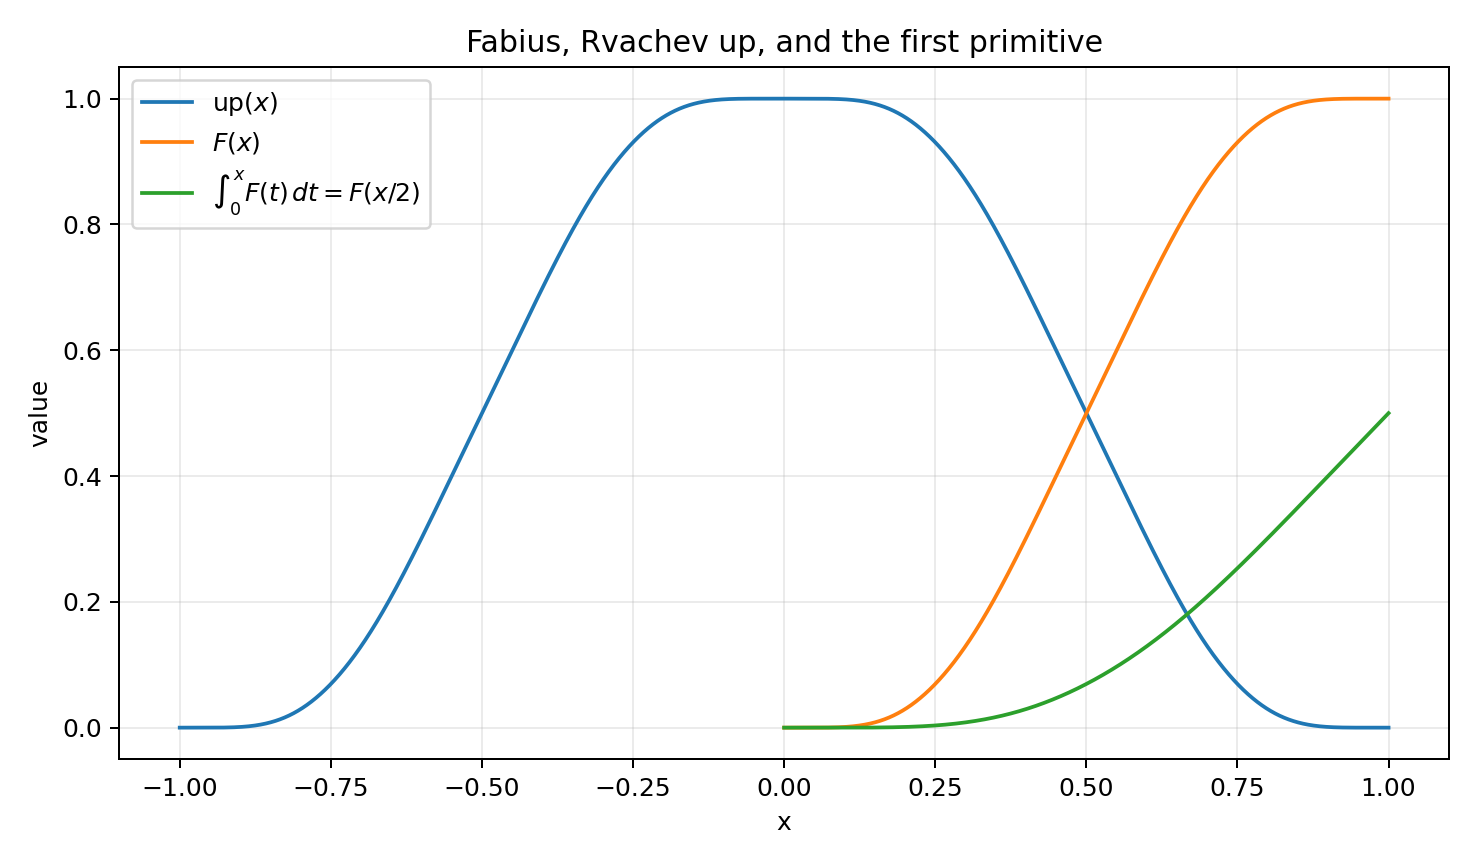
\includegraphics[width=0.92\textwidth]{functions_and_primitives.png}
 \caption{The Fabius function, Rvachev's \(\upf\)-function, and the exact first primitive
 \(\int_0^xF(t)\dd t=F(x/2)\).}
 \label{fig:functions}
\end{figure}

\subsection{Representative checks}

\begin{table}[ht]
\centering
\small
\begin{tabular}{lll}
\toprule
Identity & Test range & observed discrepancy \\
\midrule
Integer primitive ladder for \(F\) & orders \(1\) through \(5\) & below \(4\times10^{-11}\) \\
Integer primitive ladder for \(\upf\) & orders \(1\) through \(5\) & below \(8\times10^{-11}\) \\
Complex-power series, \(\alpha=-1.5\) & 100 terms at \(x=0.73\) & \(1.6\times10^{-7}\) \\
Complex-power series, \(\alpha=0.5\) & 100 terms at \(x=0.73\) & \(1.3\times10^{-10}\) \\
Laplace products & four real/complex points & below \(3\times10^{-15}\) \\
Mellin series, \(z=1+2\ii\) & 321 moments & \(2.4\times10^{-16}\) \\
Derivative pushforward moments & orders \(1\) through \(6\) & below \(2.1\times10^{-12}\) \\
Inverse primitive & five \(y\)-values & about \(3.7\times10^{-8}\) \\
Inverse exponential/Stieltjes transforms & four complex tests & below \(3.5\times10^{-8}\) \\
\bottomrule
\end{tabular}
\caption{Numerical verification.  The larger inverse-primitive discrepancy comes from
linear inversion of a finite grid, not from the closed formula.}
\label{tab:numerics}
\end{table}

The computed nonlinear constants include
\begin{align}
 \int_0^1F(x)^2\dd x&=0.404436767983985\ldots,             \label{eq:F2-num}\\
 \int_0^1F(x)^3\dd x&=0.356655151975978\ldots,             \\
 \int_{-1}^1\upf(x)^2\dd x&=0.808873535967971\ldots.      \label{eq:up2-num}
\end{align}

\begin{figure}[ht]
 \centering
 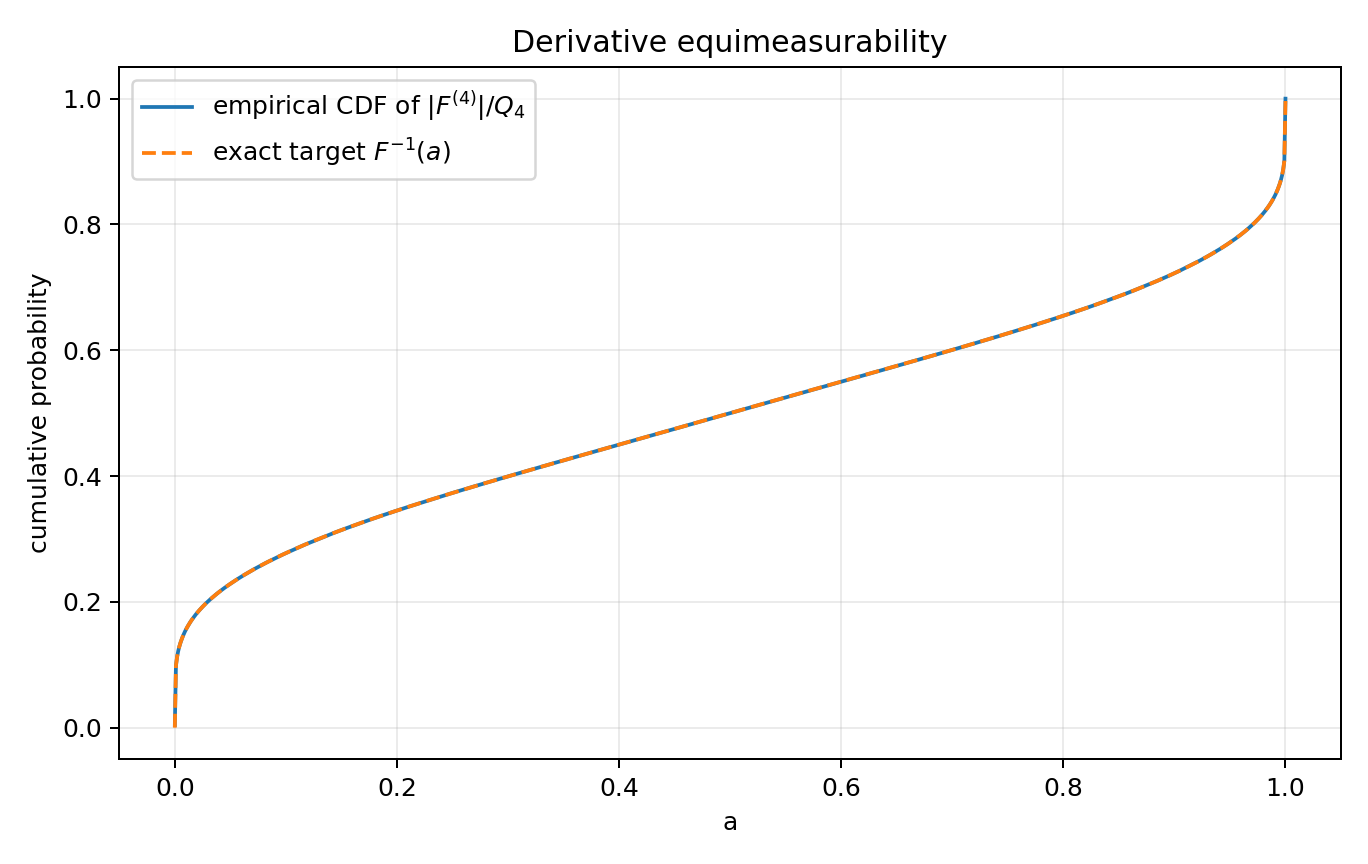
\includegraphics[width=0.82\textwidth]{pushforward_cdf.png}
 \caption{The empirical CDF of \(\abs{F^{(4)}}/Q_4\) lies on the exact target
 \(I=F^{-1}\), illustrating \cref{thm:pushforward}.}
 \label{fig:pushforward}
\end{figure}

\begin{figure}[ht]
 \centering
 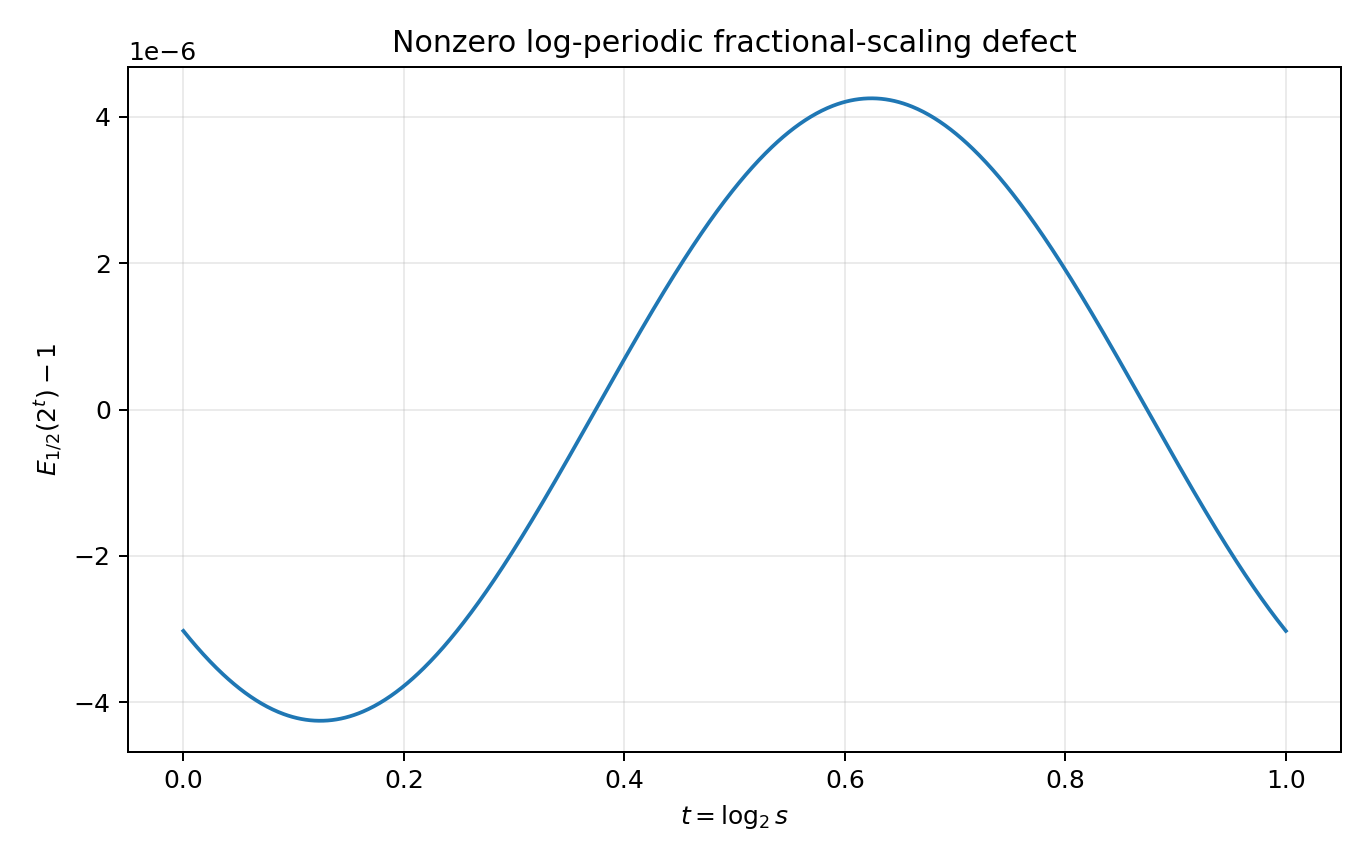
\includegraphics[width=0.82\textwidth]{fractional_defect.png}
 \caption{One logarithmic period of the nonzero defect
 \(P(t-1/2)/P(t)-1\).  Its parts-per-million size makes the false fractional scaling law
 numerically seductive.}
 \label{fig:fractional-defect}
\end{figure}

\clearpage
\section{Further conjectures and research directions}

\subsection{Higher inverse derivatives}

The sharp threshold in \cref{conj:higher-inverse-Lp} is the most immediate analytic
problem.  A proof should combine:
\begin{enumerate}
  \item the exact recursion \eqref{eq:inverse-derivative-recursion};
  \item the all-orders Lambert--\(W\) expansion for \(F\) and \(F'\) near zero;
  \item a noncancellation theorem for the leading inverse Bell polynomial;
  \item symmetry to transfer the result to \(y\uparrow1\).
\end{enumerate}
A successful proof would determine the precise Lorentz endpoint space and may reveal a
log-periodic refinement at \(p=1/n\).

\subsection{Growth and zeros of the entire inverse-moment function}

\begin{conjecture}[Order-two, log-periodically modulated growth]
The entire function \(D(z)=\int_0^1I(y)^z\dd y\) has order two.  Along the negative
real axis,
\begin{equation}
 \log D(-r)=\frac{\log2}{2}r^2+O(r\log r),                \label{eq:D-order-conj}
\end{equation}
with a nonconstant periodic correction in the natural dyadic saddle phase.  Its complex
zero counting function should inherit the same order and a dyadic modulation.
\end{conjecture}

This should be approachable by applying the repository's endpoint saddle machinery to
the Mellin integral defining \(D(-r)\).  The exact series \eqref{eq:D-series} gives an
independent Newton/binomial route and a stringent numerical cross-check.

\subsection{Arithmetic nature of singular integrals}

The constants
\begin{equation}
 D(-m),\qquad H(-m)=\frac{D(-m)-1}{m},\qquad
 D^{(r)}(0)                                                \label{eq:arithmetic-constants}
\end{equation}
are explicit convergent series of rational Rvachev moments, but their arithmetic nature
is unknown.  It is reasonable to ask whether any are rational, algebraic, or provably
transcendental.  Their dyadic product origin suggests connections with Mahler functions
and special values of \(q\)-products, but the entire interpolation does not appear to be
a standard Mahler function in \(z\).

\subsection{Fractional primitive linear independence}

\begin{conjecture}[No finite scaled-Fabius representation at noninteger order]
For \(\beta\notin\N\), the causal fractional primitive \(U_\beta\) in
\eqref{eq:fractional-up} cannot be represented on a nonempty interval as a finite linear
combination of affine-scaled copies of \(F\), \(1-F\), or \(\upf\) with algebraic
coefficient functions.
\end{conjecture}

\Cref{thm:fractional-obstruction} proves the simplest one-term global version.  A finite
combination would imply a finite exponential-polynomial relation among shifted periodic
factors in Laplace space; nonvanishing of all Fourier modes is a promising route to
linear independence.

\subsection{Dyadic autocorrelations and \(q\)-arithmetic}

The values \(\mathcal R(k/2^n)\) mix two shifted Fabius pieces.  A useful program is to:
\begin{itemize}
  \item derive a finite-scale recursion for dyadic autocorrelations from the random fixed
        point \eqref{eq:random-fixed-point};
  \item express the result through sinc-square products and Thue--Morse blocks;
  \item determine whether any nontrivial dyadic shifts have rational or controlled
        \(2\)-adic values;
  \item connect the recursion to the exact \(q\)-binomial arrays already formalized.
\end{itemize}
The integer relation \(\mathcal R(0)+2\mathcal R(1)=1\) is the first boundary datum.

\subsection{Formalization roadmap}

At compiled checkpoint \texttt{e109088ed}, the generic affine, base-point-change, and
zero-tail polynomial calculus in
\cref{eq:lean-affine-current,eq:lean-comp-affine-current,eq:lean-basepoint-current,eq:lean-zero-tail-current}
is no longer a roadmap item, and the signed-global and bounded-\(F\) natural-monomial
coefficients are formalized separately.  The remaining Lean-ready work is more narrowly:
\begin{enumerate}
  \item add narrowly packaged specializations for the report's \(1-F\), shifted-\(\upf\),
        and exterior piecewise moment-coefficient formulas, without reproving the generic
        Volterra layer or the already formalized signed/bounded \(F\) cases;
  \item the inverse primitive, by change of variables and integration by parts;
  \item the pushforward theorem, by a finite block partition and Thue--Morse balance;
  \item the inverse \(L^p\) identity and divergence threshold;
  \item the beta-chain and Bell-polynomial integral identities.
\end{enumerate}
The Mellin-entire extension and fractional obstruction require more analytic
infrastructure but have short conceptual proofs once local uniform convergence and the
periodic Laplace factor are available.

\section{Conclusion}

The self-differential identity does considerably more than generate derivatives.  With
the correct zero-initial normalization it creates an exact two-sided integer calculus,
and this calculus survives multiplication by polynomials in a finite form and by complex
powers in a convergent infinite form.  The inverse function is equally rigid: its first
primitive is closed in terms of one scaled Fabius value, all integer powers have finite
primitives, and every complex inverse moment lies on one entire binomial-moment
interpolant.

The derivative pushforward theorem reveals a hidden conservation law: after removal of
the triangular factor \(Q_m\), every derivative magnitude has exactly the same value
distribution.  This collapses infinitely many norm computations to one base integral
and gives the sharp Sobolev failure of the inverse.  Finally, the tiny nonconstant
log-periodic factor explains both the near-validity and the exact failure of naive
fractional self-similarity.

These results open a coherent frontier joining antiderivatives, quantiles, integral
transforms, dyadic arithmetic, Thue--Morse signs, Bell polynomials, and Lambert--\(W\)
asymptotics.  The remaining formal targets are the report-specific and analytic statements
not covered by the compiled generic Volterra layer.

\appendix
\section{Corpus map used in the audit}

The recursive repository material was grouped as follows.

\begin{longtable}{>{\raggedright\arraybackslash}p{0.29\textwidth}>{\raggedright\arraybackslash}p{0.61\textwidth}}
\toprule
Corpus component & Role in the audit \\
\midrule
\endhead
\path{Fabius_Function_and_Rvachev_Up} &
Current foundational exposition: definitions, derivative orbit, moments, probability,
Fourier product, exact arithmetic, and asymptotics. \\
\texttt{non-formalized-}\linebreak\texttt{research-frontiers} &
Canonical merged frontier synthesis: dyadic formula web, asymptotic completion,
Thue--Morse rates, periodic Laplace factors, and research-status boundaries. \\
Inverse frontier report &
Inverse germs, reversion, endpoint inversion, and Lambert--\(W\) corrections; checked to
separate the new inverse integral identities from existing local inverse series. \\
Newton--Rvachev frontier report &
Generalized scale sequences, Newton products, Mellin endpoint poles, and a recursive
67-source ledger. \\
Fourier-decay draft family &
Sharp decay of the infinite sinc product and periodic corrections; used to avoid
restating spectral asymptotics as new integral results. \\
Thue--Morse and dyadic arithmetic reports &
Exact sign blocks, \(q\)-binomial identities, interpolation, and rational dyadic values;
used in the block proof and the rational-integral corollary. \\
Repeated-integration reports and archive &
Approximation of \(\upf\) by iterative integration; distinguished from the exact
antiderivatives of the limiting function developed here. \\
Papers and transcriptions &
Fabius, Rvachev, Arias de Reyna, Haugland, and related primary/background sources. \\
Lean walkthrough and glossary &
Notation, formal dependencies, and theorem naming. \\
\bottomrule
\end{longtable}

Searches for \emph{antiderivative}, \emph{equimeasurable}, inverse \(L^p\) laws, and the
specific Mellin identity \eqref{eq:inverse-mellin} returned no developed counterpart in
the current canonical volumes or live inverse report.  Existing moment and transform
formulae have been credited as inputs wherever they are reused.

\section{Selected formulas for direct use}

For convenience, the main computational identities are collected here.

\begin{align*}
 \Iop^nF(x)&=2^{n(n-1)/2}F(x/2^n),\\
 \Iop^n\upf(x)&=2^{n(n-1)/2}F((x+1)/2^n),\quad -1\le x\le1,\\
 \Iop^n(PF)(x)&=\sum_{k=0}^{\deg P}(-1)^k\binom{n+k-1}{k}
 P^{(k)}(x)2^{(n+k)(n+k-1)/2}F(x/2^{n+k}),\\
 \int_0^yI(v)\dd v&=yI(y)-F(I(y)/2),\\
 \int_0^1I(y)^z\dd y&=2^{-z}\sum_{j\ge0}\binom z{2j}c_j,\\
 \int_0^1e^{sI(y)}\dd y&=e^{s/2}M(s/2),\\
 \int_0^1\frac{\dd y}{z-I(y)}&=2C(2z-1),\\
 \int_0^1\Phi(\abs{F^{(m)}}/Q_m)\dd x&=\int_0^1\Phi(F)\dd x,\\
 \int_0^1I'(y)^p\dd y&=2^{1-p}\int_0^1F(x)^{1-p}\dd x\quad(p\le1),\\
 \int_0^1e^{sx}F(x)\dd x&=\frac{e^s-e^{s/2}M(s/2)}s,\\
 \Lap[U_\beta(\cdot-1)](s)&=s^{-\beta}e^{-s}M(s).
\end{align*}

\section{Reproducibility files}

The archive accompanying this report contains:
\begin{itemize}
 \item \texttt{fabius\_integral\_frontiers.tex} --- this source;
 \item \texttt{fabius\_integral\_frontiers.pdf} --- the rendered report;
 \item \texttt{numerical\_experiments.py} --- commented FFT and quadrature code;
 \item \texttt{numerical\_results.txt} --- machine-generated numerical output;
 \item three PNG figures used in the report.
\end{itemize}
The script fixes no random seed because it uses deterministic quadrature and
Fourier inversion rather than Monte Carlo sampling.

\begin{thebibliography}{99}

\bibitem{Arias1982}
J. Arias de Reyna,
\emph{An infinitely differentiable function with compact support: definition and
properties}, Rev. Real Acad. Ciencias Madrid 76 (1982), 21--38; English translation,
\href{https://arxiv.org/abs/1702.05442}{arXiv:1702.05442}.

\bibitem{Arias2018}
J. Arias de Reyna,
\emph{Arithmetic of the Fabius function}, Integers 18 (2018), Paper A51;
\href{https://arxiv.org/abs/1702.06487}{arXiv:1702.06487}.

\bibitem{Fabius1966}
J. Fabius,
\emph{A probabilistic example of a nowhere analytic \(C^\infty\)-function},
Z. Wahrscheinlichkeitstheorie verw. Gebiete 5 (1966), 173--174,
\href{https://doi.org/10.1007/BF00536652}{doi:10.1007/BF00536652}.

\bibitem{Rvachev1990}
V. A. Rvachev,
\emph{Compactly supported solutions of functional-differential equations and their
applications}, Russian Math. Surveys 45:1 (1990), 87--120,
\href{https://doi.org/10.1070/RM1990v045n01ABEH002324}{doi:10.1070/RM1990v045n01ABEH002324}.

\bibitem{ProveItMain}
V. Reshetnikov,
\emph{The Fabius Function and Rvachev's Up-Function: exact arithmetic, probability,
Fourier analysis, and corrected sharp asymptotics}, current LaTeX monograph in the
\href{https://github.com/VladimirReshetnikov/ProveIt/tree/main/Analysis/FabiusFunction/docs}{ProveIt repository}.

\bibitem{ProveItFrontiers}
V. Reshetnikov,
\emph{Non-Formalized Research Frontiers for the Fabius Function: six thematic
syntheses awaiting Lean verification}, current unified frontier volume in the
\href{https://github.com/VladimirReshetnikov/ProveIt/tree/main/Analysis/FabiusFunction/docs/non-formalized-research-frontiers}{ProveIt repository}.

\bibitem{Samko}
S. G. Samko, A. A. Kilbas, and O. I. Marichev,
\emph{Fractional Integrals and Derivatives: Theory and Applications}, Gordon and
Breach, 1993.

\bibitem{Comtet}
L. Comtet,
\emph{Advanced Combinatorics}, Reidel, 1974.

\bibitem{DLMF}
NIST Digital Library of Mathematical Functions,
\emph{Mellin transform methods}, \href{https://dlmf.nist.gov/2.5}{DLMF \S2.5}.

\end{thebibliography}

\end{document}
